\documentclass[]{book}
\usepackage{lmodern}
\usepackage{amssymb,amsmath}
\usepackage{ifxetex,ifluatex}
\usepackage{fixltx2e} % provides \textsubscript
\ifnum 0\ifxetex 1\fi\ifluatex 1\fi=0 % if pdftex
  \usepackage[T1]{fontenc}
  \usepackage[utf8]{inputenc}
\else % if luatex or xelatex
  \ifxetex
    \usepackage{mathspec}
  \else
    \usepackage{fontspec}
  \fi
  \defaultfontfeatures{Ligatures=TeX,Scale=MatchLowercase}
\fi
% use upquote if available, for straight quotes in verbatim environments
\IfFileExists{upquote.sty}{\usepackage{upquote}}{}
% use microtype if available
\IfFileExists{microtype.sty}{%
\usepackage{microtype}
\UseMicrotypeSet[protrusion]{basicmath} % disable protrusion for tt fonts
}{}
\usepackage[margin=1in]{geometry}
\usepackage{hyperref}
\hypersetup{unicode=true,
            pdftitle={Uncertainty Visualization},
            pdfauthor={Matthew Kay},
            pdfborder={0 0 0},
            breaklinks=true}
\urlstyle{same}  % don't use monospace font for urls
\usepackage{natbib}
\bibliographystyle{apalike}
\usepackage{color}
\usepackage{fancyvrb}
\newcommand{\VerbBar}{|}
\newcommand{\VERB}{\Verb[commandchars=\\\{\}]}
\DefineVerbatimEnvironment{Highlighting}{Verbatim}{commandchars=\\\{\}}
% Add ',fontsize=\small' for more characters per line
\usepackage{framed}
\definecolor{shadecolor}{RGB}{248,248,248}
\newenvironment{Shaded}{\begin{snugshade}}{\end{snugshade}}
\newcommand{\AlertTok}[1]{\textcolor[rgb]{0.94,0.16,0.16}{#1}}
\newcommand{\AnnotationTok}[1]{\textcolor[rgb]{0.56,0.35,0.01}{\textbf{\textit{#1}}}}
\newcommand{\AttributeTok}[1]{\textcolor[rgb]{0.77,0.63,0.00}{#1}}
\newcommand{\BaseNTok}[1]{\textcolor[rgb]{0.00,0.00,0.81}{#1}}
\newcommand{\BuiltInTok}[1]{#1}
\newcommand{\CharTok}[1]{\textcolor[rgb]{0.31,0.60,0.02}{#1}}
\newcommand{\CommentTok}[1]{\textcolor[rgb]{0.56,0.35,0.01}{\textit{#1}}}
\newcommand{\CommentVarTok}[1]{\textcolor[rgb]{0.56,0.35,0.01}{\textbf{\textit{#1}}}}
\newcommand{\ConstantTok}[1]{\textcolor[rgb]{0.00,0.00,0.00}{#1}}
\newcommand{\ControlFlowTok}[1]{\textcolor[rgb]{0.13,0.29,0.53}{\textbf{#1}}}
\newcommand{\DataTypeTok}[1]{\textcolor[rgb]{0.13,0.29,0.53}{#1}}
\newcommand{\DecValTok}[1]{\textcolor[rgb]{0.00,0.00,0.81}{#1}}
\newcommand{\DocumentationTok}[1]{\textcolor[rgb]{0.56,0.35,0.01}{\textbf{\textit{#1}}}}
\newcommand{\ErrorTok}[1]{\textcolor[rgb]{0.64,0.00,0.00}{\textbf{#1}}}
\newcommand{\ExtensionTok}[1]{#1}
\newcommand{\FloatTok}[1]{\textcolor[rgb]{0.00,0.00,0.81}{#1}}
\newcommand{\FunctionTok}[1]{\textcolor[rgb]{0.00,0.00,0.00}{#1}}
\newcommand{\ImportTok}[1]{#1}
\newcommand{\InformationTok}[1]{\textcolor[rgb]{0.56,0.35,0.01}{\textbf{\textit{#1}}}}
\newcommand{\KeywordTok}[1]{\textcolor[rgb]{0.13,0.29,0.53}{\textbf{#1}}}
\newcommand{\NormalTok}[1]{#1}
\newcommand{\OperatorTok}[1]{\textcolor[rgb]{0.81,0.36,0.00}{\textbf{#1}}}
\newcommand{\OtherTok}[1]{\textcolor[rgb]{0.56,0.35,0.01}{#1}}
\newcommand{\PreprocessorTok}[1]{\textcolor[rgb]{0.56,0.35,0.01}{\textit{#1}}}
\newcommand{\RegionMarkerTok}[1]{#1}
\newcommand{\SpecialCharTok}[1]{\textcolor[rgb]{0.00,0.00,0.00}{#1}}
\newcommand{\SpecialStringTok}[1]{\textcolor[rgb]{0.31,0.60,0.02}{#1}}
\newcommand{\StringTok}[1]{\textcolor[rgb]{0.31,0.60,0.02}{#1}}
\newcommand{\VariableTok}[1]{\textcolor[rgb]{0.00,0.00,0.00}{#1}}
\newcommand{\VerbatimStringTok}[1]{\textcolor[rgb]{0.31,0.60,0.02}{#1}}
\newcommand{\WarningTok}[1]{\textcolor[rgb]{0.56,0.35,0.01}{\textbf{\textit{#1}}}}
\usepackage{longtable,booktabs}
\usepackage{graphicx,grffile}
\makeatletter
\def\maxwidth{\ifdim\Gin@nat@width>\linewidth\linewidth\else\Gin@nat@width\fi}
\def\maxheight{\ifdim\Gin@nat@height>\textheight\textheight\else\Gin@nat@height\fi}
\makeatother
% Scale images if necessary, so that they will not overflow the page
% margins by default, and it is still possible to overwrite the defaults
% using explicit options in \includegraphics[width, height, ...]{}
\setkeys{Gin}{width=\maxwidth,height=\maxheight,keepaspectratio}
\IfFileExists{parskip.sty}{%
\usepackage{parskip}
}{% else
\setlength{\parindent}{0pt}
\setlength{\parskip}{6pt plus 2pt minus 1pt}
}
\setlength{\emergencystretch}{3em}  % prevent overfull lines
\providecommand{\tightlist}{%
  \setlength{\itemsep}{0pt}\setlength{\parskip}{0pt}}
\setcounter{secnumdepth}{5}
% Redefines (sub)paragraphs to behave more like sections
\ifx\paragraph\undefined\else
\let\oldparagraph\paragraph
\renewcommand{\paragraph}[1]{\oldparagraph{#1}\mbox{}}
\fi
\ifx\subparagraph\undefined\else
\let\oldsubparagraph\subparagraph
\renewcommand{\subparagraph}[1]{\oldsubparagraph{#1}\mbox{}}
\fi

%%% Use protect on footnotes to avoid problems with footnotes in titles
\let\rmarkdownfootnote\footnote%
\def\footnote{\protect\rmarkdownfootnote}

%%% Change title format to be more compact
\usepackage{titling}

% Create subtitle command for use in maketitle
\newcommand{\subtitle}[1]{
  \posttitle{
    \begin{center}\large#1\end{center}
    }
}

\setlength{\droptitle}{-2em}

  \title{Uncertainty Visualization}
    \pretitle{\vspace{\droptitle}\centering\huge}
  \posttitle{\par}
    \author{Matthew Kay}
    \preauthor{\centering\large\emph}
  \postauthor{\par}
      \predate{\centering\large\emph}
  \postdate{\par}
    \date{2018-10-16}

\usepackage{booktabs}
\usepackage{amsthm}
\makeatletter
\def\thm@space@setup{%
  \thm@preskip=8pt plus 2pt minus 4pt
  \thm@postskip=\thm@preskip
}
\makeatother

\usepackage{amsthm}
\newtheorem{theorem}{Theorem}[chapter]
\newtheorem{lemma}{Lemma}[chapter]
\theoremstyle{definition}
\newtheorem{definition}{Definition}[chapter]
\newtheorem{corollary}{Corollary}[chapter]
\newtheorem{proposition}{Proposition}[chapter]
\theoremstyle{definition}
\newtheorem{example}{Example}[chapter]
\theoremstyle{definition}
\newtheorem{exercise}{Exercise}[chapter]
\theoremstyle{remark}
\newtheorem*{remark}{Remark}
\newtheorem*{solution}{Solution}
\begin{document}
\maketitle

{
\setcounter{tocdepth}{1}
\tableofcontents
}
\hypertarget{preface}{%
\chapter*{Preface}\label{preface}}
\addcontentsline{toc}{chapter}{Preface}

This book\footnote{or what it will be---it is a work in progress} aims
to provide the \emph{why} and the \emph{how} of uncertainty
visualization. The \emph{why} is based on what we currently know about
how people interpret and make decisions from uncertainty visualizations,
and the \emph{how} is structured around generating uncertainty
visualizations using the R programming language and the grammar of
graphics.\footnote{as implemented in the \emph{ggplot2} package
  \citep{R-ggplot2}}

\hypertarget{ch-intro}{%
\chapter{Introduction}\label{ch-intro}}

TBD

\hypertarget{ch-why-hard}{%
\chapter{Why uncertainty visualization is hard}\label{ch-why-hard}}

\begin{itemize}
\tightlist
\item
  Efficient encodings for uncertainty can be hard to find

  \begin{itemize}
  \tightlist
  \item
    try putting mean, variance, and interval estimation in one plot +
    doing this when useful channels are already used up
  \end{itemize}
\item
  Even if you get the encoding right have to contend with making sure
  people understand it

  \begin{itemize}
  \tightlist
  \item
    explain a CDF to someone (N.B.: sometimes this works! task has an
    effect here)
  \end{itemize}
\item
  Even if people understand have to deal with how people perceive
  uncertainty

  \begin{itemize}
  \tightlist
  \item
    linear-in-log-odds and other perceptual models of probability
  \end{itemize}
\item
  Even if people correctly perceive the uncertainty have to deal with
  how people make decisions under uncertainty
\item
  Even if you solve all these problems in one context a new context may
  cause your solution to break

  \begin{itemize}
  \tightlist
  \item
    see e.g.~deterministic construal errors
  \end{itemize}
\item
  Plus, you still have to build the damn thing

  \begin{itemize}
  \tightlist
  \item
    But some strategies for building uncertainty vis using the grammar
    of graphics helps a lot here (the \textbf{how} of this book)
  \end{itemize}
\end{itemize}

\hypertarget{ch-uncertainty}{%
\chapter{Foundations: Uncertainty as we'll see
it}\label{ch-uncertainty}}

\begin{itemize}
\tightlist
\item
  primarily Bayesian perspective

  \begin{itemize}
  \tightlist
  \item
    unifies aleatory and epistemic
  \item
    gives us one framework to work in
  \item
    simplifies building things
  \item
    simplifies communicating things (see e.g.~confidence fallacy)
  \end{itemize}
\item
  will still occasionally touch on frequentist, usually as a subsection
  at the end of each chapter:

  \begin{itemize}
  \tightlist
  \item
    tips on how to translate the visualization techniques presented into
    that mode
  \item
    at times, visualizations unique to the frequentist approach that
    might be useful
  \end{itemize}
\end{itemize}

\hypertarget{ch-vis-foundations}{%
\chapter{Foundations: Uncertainty and the grammar of
graphics}\label{ch-vis-foundations}}

\begin{itemize}
\tightlist
\item
  basic strategies for applying uncertainty visualization within the
  grammar of graphics
\item
  visual channels, marks, etc. (and mapping onto ggplot)
\item
  simple prediction grid example
\end{itemize}

\hypertarget{ch-strategies}{%
\chapter{Foundations: General strategies}\label{ch-strategies}}

\emph{Dunno if this goes before or after all the specific examples}

\begin{itemize}
\tightlist
\item
  think about task

  \begin{itemize}
  \tightlist
  \item
    what do people actually need from the representation to do the task?
    densities? intervals? (arbitrary or known in advance?) point
    estimates?
  \end{itemize}
\item
  employ frequency framing where possible

  \begin{itemize}
  \tightlist
  \item
    \emph{(maybe a table here translating common non-frequency
    representations into frequency representations)}
  \item
    quantile dotplots
  \item
    representative sampling in scatterplots (need a better name for
    this)
  \item
    spaghettis
  \item
    pixelated maps (also needs a name)
  \end{itemize}
\item
  use animation / HOPs
\item
  anticipate deterministic construal errors

  \begin{itemize}
  \tightlist
  \item
    think about task context, common elements of that context with
    plausibly similar abstract representations
  \item
    when animating / using metaphor, think about the mechanism - do we
    think of it as random?
  \end{itemize}
\end{itemize}

\hypertarget{ch-discrete}{%
\chapter{Discrete data}\label{ch-discrete}}

\begin{itemize}
\tightlist
\item
  categorical

  \begin{itemize}
  \tightlist
  \item
    proportions

    \begin{itemize}
    \tightlist
    \item
      product plots / mosaic plots
    \end{itemize}
  \item
    icon arrays

    \begin{itemize}
    \tightlist
    \item
      unit visualizations
    \end{itemize}
  \item
    HOPs-like stuff
  \item
    entropy-based approaches
  \end{itemize}
\item
  ordinal / integer

  \begin{itemize}
  \tightlist
  \item
    proportions
  \item
    histograms
  \item
    CDFs
  \item
    dotplots
  \item
    \ldots{}
  \end{itemize}
\end{itemize}

\hypertarget{ch-continuous}{%
\chapter{Continuous data}\label{ch-continuous}}

\emph{not sure of the organization here, especially within
multivariate\ldots{}}

\begin{itemize}
\tightlist
\item
  univariate

  \begin{itemize}
  \tightlist
  \item
    densities, gradients
  \item
    CDFs
  \item
    intervals
  \item
    quantile dotplots
  \item
    HOPs
  \end{itemize}
\item
  multivariate

  \begin{itemize}
  \tightlist
  \item
    the joint case

    \begin{itemize}
    \tightlist
    \item
      gradients
    \item
      contour plots
    \end{itemize}
  \item
    the conditional case

    \begin{itemize}
    \tightlist
    \item
      gradients
    \item
      bands
    \end{itemize}
  \item
    generalizing quantile dotplots to multiple dimensions:
    representative sampling approaches

    \begin{itemize}
    \tightlist
    \item
      scatterplots
    \item
      spaghetti plots
    \end{itemize}
  \item
    HOPs
  \end{itemize}
\item
  frequentist addendum

  \begin{itemize}
  \tightlist
  \item
    interpreting in a Bayesian mode: advantages and pitfalls (and what
    it reveals)

    \begin{itemize}
    \tightlist
    \item
      \emph{this maybe goes elsewhere}
    \end{itemize}
  \item
    those double-sided p value plot things
  \end{itemize}
\end{itemize}

\hypertarget{ch-multiple}{%
\chapter{Dealing with multiple uncertainties}\label{ch-multiple}}

\begin{itemize}
\tightlist
\item
  a note on comparisons

  \begin{itemize}
  \tightlist
  \item
    univariate marginals might bite you\ldots{}
  \end{itemize}
\item
  aleatory / epistemic (or data space / parameter space)

  \begin{itemize}
  \tightlist
  \item
    frankenplots maybe (product plots / mosaic plots / unit
    visualizations)
  \item
    animation

    \begin{itemize}
    \tightlist
    \item
      NYT needle
    \item
      Galton boards
    \end{itemize}
  \end{itemize}
\item
  mixing discrete and continuous

  \begin{itemize}
  \tightlist
  \item
    color with densities
  \item
    HOPs
  \item
    some hurricane stuff
  \end{itemize}
\end{itemize}

\hypertarget{ch-maps-glyphs}{%
\chapter{Maps and glyphs}\label{ch-maps-glyphs}}

\emph{Not sure this is a separate chapter but putting this here for
now\ldots{}}

\begin{itemize}
\tightlist
\item
  always remember to ask if you need a map in the first place
\item
  uncertainty glyphs

  \begin{itemize}
  \tightlist
  \item
    blur, and problems with it
  \item
    problems with glyphs more generally
  \end{itemize}
\item
  bivariate maps
\item
  VSUPs

  \begin{itemize}
  \tightlist
  \item
    connect back to LLO and/or regularization (I think LLO\ldots{})
  \end{itemize}
\item
  pixelation
\item
  HOPs
\end{itemize}

\hypertarget{scratch-space}{%
\chapter*{Scratch space}\label{scratch-space}}
\addcontentsline{toc}{chapter}{Scratch space}

\begin{Shaded}
\begin{Highlighting}[]
\KeywordTok{library}\NormalTok{(tidyverse)}
\KeywordTok{library}\NormalTok{(modelr)}
\KeywordTok{library}\NormalTok{(broom)}
\KeywordTok{library}\NormalTok{(ggstance)}
\end{Highlighting}
\end{Shaded}

\begin{Shaded}
\begin{Highlighting}[]
\KeywordTok{set.seed}\NormalTok{(}\DecValTok{12345}\NormalTok{)}
\NormalTok{x =}\StringTok{ }\KeywordTok{rnorm}\NormalTok{(}\DecValTok{10}\NormalTok{, }\FloatTok{-0.25}\NormalTok{)}
\NormalTok{ci_color =}\StringTok{ "#d95f02"}

\NormalTok{intervals =}\StringTok{ }\KeywordTok{data_frame}\NormalTok{(}
    \CommentTok{# conf.level = seq(.7, .99, by = .01),}
    \DataTypeTok{conf.level =} \KeywordTok{c}\NormalTok{(.}\DecValTok{50}\NormalTok{, }\FloatTok{.80}\NormalTok{, }\FloatTok{.95}\NormalTok{),}
    \DataTypeTok{alpha =} \DecValTok{1} \OperatorTok{-}\StringTok{ }\NormalTok{conf.level,}
    \DataTypeTok{test =} \KeywordTok{map}\NormalTok{(conf.level, }\OperatorTok{~}\StringTok{ }\KeywordTok{tidy}\NormalTok{(}\KeywordTok{t.test}\NormalTok{(x, }\DataTypeTok{conf.level =}\NormalTok{ ..}\DecValTok{1}\NormalTok{)))}
\NormalTok{  ) }\OperatorTok
\StringTok{  }\KeywordTok{unnest}\NormalTok{()}

\KeywordTok{crossing}\NormalTok{(}
    \DataTypeTok{null =} \KeywordTok{seq}\NormalTok{(}\OperatorTok{-}\DecValTok{6}\NormalTok{, }\DecValTok{6}\NormalTok{, }\DataTypeTok{length.out =} \DecValTok{1001}\NormalTok{)}
\NormalTok{  ) }\OperatorTok
\StringTok{  }\KeywordTok{mutate}\NormalTok{(}\DataTypeTok{test =} \KeywordTok{map}\NormalTok{(null, }\OperatorTok{~}\StringTok{ }\KeywordTok{tidy}\NormalTok{(}\KeywordTok{t.test}\NormalTok{(x, }\DataTypeTok{mu =}\NormalTok{ ..}\DecValTok{1}\NormalTok{)))) }\OperatorTok
\StringTok{  }\KeywordTok{unnest}\NormalTok{() }\OperatorTok
\StringTok{  }\KeywordTok{ggplot}\NormalTok{() }\OperatorTok{+}
\StringTok{  }\KeywordTok{geom_line}\NormalTok{(}\KeywordTok{aes}\NormalTok{(}\DataTypeTok{x =}\NormalTok{ null, }\DataTypeTok{y =}\NormalTok{ p.value)) }\OperatorTok{+}
\StringTok{  }\KeywordTok{geom_hline}\NormalTok{(}\KeywordTok{aes}\NormalTok{(}\DataTypeTok{yintercept =}\NormalTok{ alpha), }\DataTypeTok{color =} \StringTok{"gray50"}\NormalTok{, }\DataTypeTok{data =}\NormalTok{ intervals, }\DataTypeTok{linetype =} \StringTok{"dotted"}\NormalTok{) }\OperatorTok{+}
\StringTok{  }\KeywordTok{geom_rect}\NormalTok{(}\KeywordTok{aes}\NormalTok{(}\DataTypeTok{xmin =}\NormalTok{ conf.low, }\DataTypeTok{xmax =}\NormalTok{ conf.high, }\DataTypeTok{ymax =}\NormalTok{ alpha), }\DataTypeTok{ymin =} \DecValTok{-1}\NormalTok{, }\DataTypeTok{fill =}\NormalTok{ ci_color, }\DataTypeTok{alpha =} \FloatTok{.1}\NormalTok{,}
    \DataTypeTok{data =}\NormalTok{ intervals, }\DataTypeTok{color =} \OtherTok{NA}\NormalTok{, }\DataTypeTok{size =} \FloatTok{.75}\NormalTok{) }\OperatorTok{+}
\StringTok{  }\KeywordTok{geom_pointrangeh}\NormalTok{(}\KeywordTok{aes}\NormalTok{(}\DataTypeTok{xmin =}\NormalTok{ conf.low, }\DataTypeTok{xmax =}\NormalTok{ conf.high, }\DataTypeTok{x =}\NormalTok{ estimate, }\DataTypeTok{y =}\NormalTok{ alpha), }
    \DataTypeTok{data =}\NormalTok{ intervals, }\DataTypeTok{color =}\NormalTok{ ci_color, }\DataTypeTok{size =} \FloatTok{.75}\NormalTok{) }\OperatorTok{+}
\StringTok{  }\KeywordTok{geom_vline}\NormalTok{(}\KeywordTok{aes}\NormalTok{(}\DataTypeTok{xintercept =}\NormalTok{ estimate), }\DataTypeTok{data =}\NormalTok{ intervals, }\DataTypeTok{color =}\NormalTok{ ci_color, }\DataTypeTok{linetype =} \StringTok{"dotted"}\NormalTok{) }\OperatorTok{+}
\StringTok{  }\KeywordTok{geom_text}\NormalTok{(}\KeywordTok{aes}\NormalTok{(}\DataTypeTok{y =}\NormalTok{ alpha, }\DataTypeTok{label =} \KeywordTok{paste0}\NormalTok{(}\StringTok{"p value = "}\NormalTok{, }\KeywordTok{format}\NormalTok{(alpha, }\DataTypeTok{digits =} \DecValTok{2}\NormalTok{, }\DataTypeTok{nsmall =} \DecValTok{2}\NormalTok{))),}
    \DataTypeTok{x =} \FloatTok{-5.3}\NormalTok{, }\DataTypeTok{vjust =} \FloatTok{-.5}\NormalTok{, }\DataTypeTok{hjust =} \DecValTok{0}\NormalTok{, }\DataTypeTok{data =}\NormalTok{ intervals, }\DataTypeTok{color =} \StringTok{"gray50"}\NormalTok{) }\OperatorTok{+}
\StringTok{  }\KeywordTok{geom_text}\NormalTok{(}\KeywordTok{aes}\NormalTok{(}\DataTypeTok{y =}\NormalTok{ alpha, }\DataTypeTok{label =} \KeywordTok{paste0}\NormalTok{(}\StringTok{"1 - "}\NormalTok{, }\KeywordTok{format}\NormalTok{(alpha, }\DataTypeTok{digits =} \DecValTok{2}\NormalTok{, }\DataTypeTok{nsmall =} \DecValTok{2}\NormalTok{), }\StringTok{" = "}\NormalTok{, }\KeywordTok{round}\NormalTok{((}\DecValTok{1} \OperatorTok{-}\StringTok{ }\NormalTok{alpha) }\OperatorTok{*}\StringTok{ }\DecValTok{100}\NormalTok{), }\StringTok{"% CI"}\NormalTok{)),}
    \DataTypeTok{x =} \FloatTok{0.33}\NormalTok{, }\DataTypeTok{vjust =} \FloatTok{-.5}\NormalTok{, }\DataTypeTok{color =}\NormalTok{ ci_color, }\DataTypeTok{hjust =} \DecValTok{0}\NormalTok{, }\DataTypeTok{data =}\NormalTok{ intervals) }\OperatorTok{+}
\StringTok{  }\KeywordTok{theme_light}\NormalTok{() }\OperatorTok{+}
\StringTok{  }\KeywordTok{theme}\NormalTok{(}\DataTypeTok{panel.grid =} \KeywordTok{element_blank}\NormalTok{()) }\OperatorTok{+}
\StringTok{  }\KeywordTok{xlab}\NormalTok{(}\StringTok{"two-sided null hypothesis"}\NormalTok{) }\OperatorTok{+}
\StringTok{  }\KeywordTok{ylab}\NormalTok{(}\StringTok{"p value"}\NormalTok{) }\OperatorTok{+}
\StringTok{  }\KeywordTok{coord_cartesian}\NormalTok{(}\DataTypeTok{xlim =} \KeywordTok{c}\NormalTok{(}\OperatorTok{-}\DecValTok{5}\NormalTok{, }\DecValTok{5}\NormalTok{))}
\end{Highlighting}
\end{Shaded}

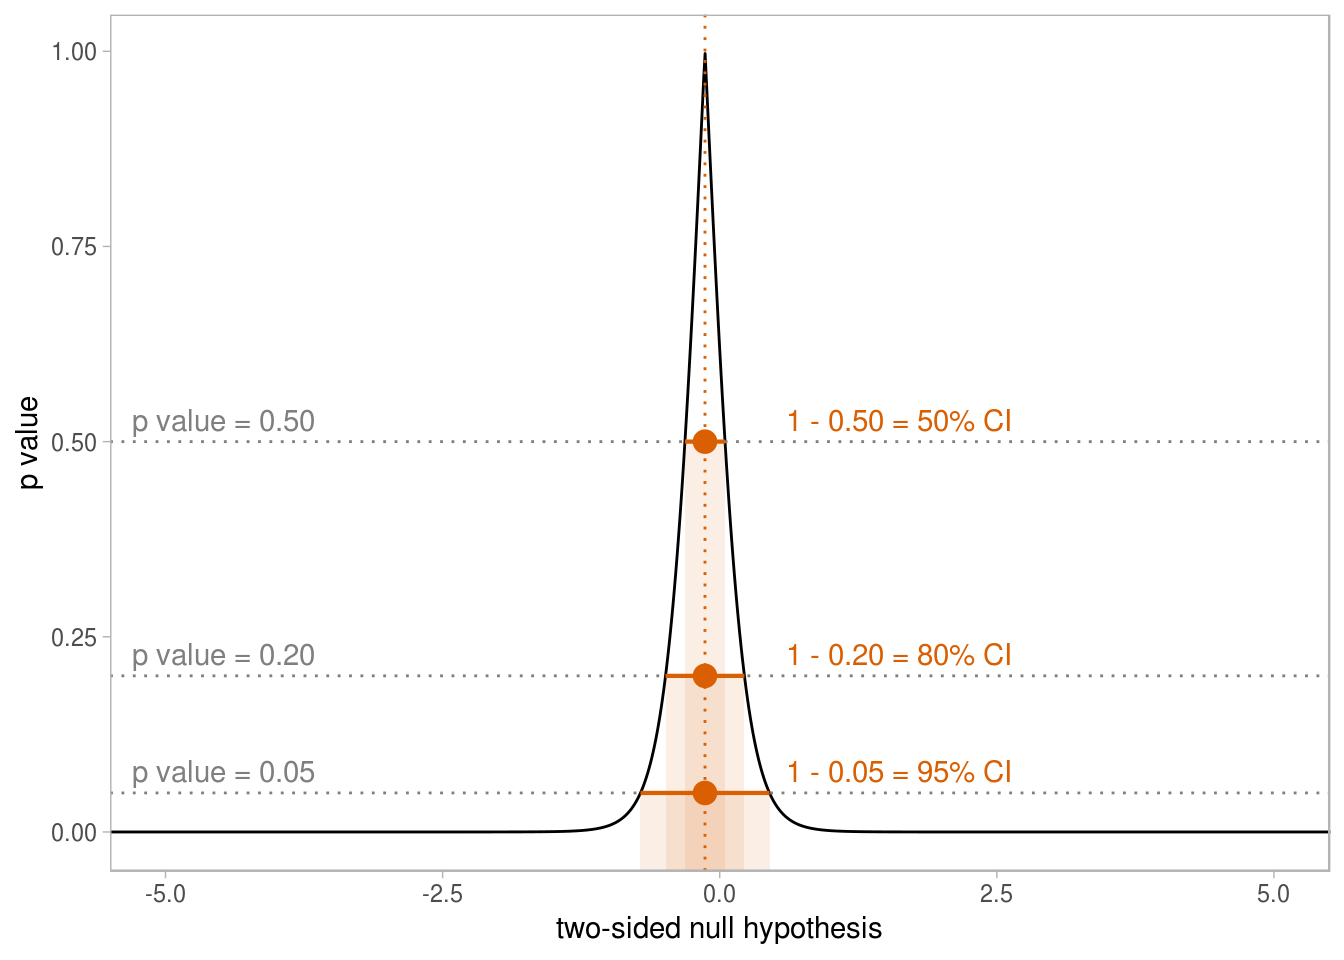
\includegraphics{uncertainty-visualization_files/figure-latex/unnamed-chunk-3-1.pdf}

\bibliography{book.bib,packages.bib}


\end{document}
